\documentclass[preprint,12pt]{elsarticle}

    \usepackage[sc]{mathpazo} % Use the Palatino font
    \usepackage[T1]{fontenc} % Use 8-bit encoding that has 256 glyphs
    \usepackage{microtype} % Slightly tweak font spacing for aesthetics
    \usepackage[english]{babel} % Language hyphenation and typographical rules
    \usepackage{booktabs} % Horizontal rules in tables
    \usepackage{enumitem} % Customized lists
    \usepackage[table,xcdraw]{xcolor}
    \usepackage[utf8]{inputenc} % Required for inputting international characters
    \usepackage{parskip}
    \usepackage{graphicx}
    \usepackage{hyperref}
    \usepackage{pdfpages}
    \usepackage{amsmath}
    \usepackage{esvect}
    \usepackage{listings}
    \usepackage{color}
    \usepackage{spverbatim}
    \usepackage{subcaption}
    \usepackage[title]{appendix}
    \hypersetup{
        colorlinks=true,
        linkcolor=blue,
        filecolor=magenta,      
        urlcolor=cyan,
    }
    \definecolor{dkgreen}{rgb}{0,0.6,0}
    \definecolor{gray}{rgb}{0.5,0.5,0.5}
    \definecolor{mauve}{rgb}{0.58,0,0.82}
    \definecolor{lightgray}{rgb}{0.83, 0.83, 0.83}
    \definecolor{timberwolf}{rgb}{0.86, 0.84, 0.82}
    \definecolor{whitesmoke}{rgb}{0.96, 0.96, 0.96}
    
    \lstset{frame=tb,
    language=python,
    aboveskip=3mm,
    belowskip=3mm,
    showstringspaces=false,
    columns=flexible,
    basicstyle={\small\ttfamily},
    numbers=none,
    numberstyle=\tiny\color{gray},
    keywordstyle=\color{blue},
    commentstyle=\color{dkgreen},
    stringstyle=\color{mauve},
    breaklines=true,
    breakatwhitespace=true,
    tabsize=3,
    backgroundcolor = \color{whitesmoke}
    }

    \begin{document}
    \title{\LARGE \bf
        STAT 391 Homework 2
        }
        
        \author{ \parbox{3 in}{\centering Chongyi Xu \\
                 University of Washington\\
                 STAT 391 Spring 2018\\
                 {\tt\small chongyix@uw.edu}}
        }
    \maketitle

    \section{Problem 1 - Estimation of small probabilities}
    \begin{enumerate}[label=\alph*]
        \item Estimate $\hat{\theta_a},\hat{\theta_b},\cdots \hat{\theta_z}$ from the given text
        I bascially use the same setup as I did for HW1 Question 4. The only difference is that I
        used $\theta^{M\ L} = 0$ for those letters that never appear. 
        \begin{lstlisting}
import math

# Helper Methods
def langReader(file):
    '''
    langReader is used to read in files and compute for the probability
    for each letter

    Args:
        file: The name of the file containing the letter and probability.
    Returns:
        A dictionary containing letters as keys and probability as values
    '''
    pLang = {}
    for line in open(file):
        el = line.split(' ')
        letter = el[1].lower()
        pLang[letter] = float(el[2])/1000
    return pLang

def LetterCounter(testString):
    '''
    Counts for the number of each letter in the test string (sufficient statistics)

    Args:
        testString: The string to count
    Returns:
        A dictionary containing letters as keys and count number as values
    '''
    counter = {}
    for char in testString:
        try:
            counter[char] = counter[char] + 1
        except KeyError:
            counter[char] = 1
    return counter

# Initialize the probability map
path = r'C:\Users\johnn\Documents\UW\SchoolWorks\2018Spring\STAT391\HW1'

english = langReader(path + r'\english.dat')

# Read in lincoln_text.txt
txt = ''
for line in open(path + r'\lincoln_text.txt'):
    txt = txt + line
txt = ''.join(e for e in txt if e.isalnum()).lower()
counter = LetterCounter(txt)
length = len(txt)

# Since there might be some missing letters
lincolnEng = {}
for letter in english:
    if letter not in counter:
        counter[letter] = 0
    lincolnEng[letter] = counter[letter] / length
print(lincolnEng)
        \end{lstlisting}
        As the result, I got my $\hat{\theta}$ to be
        \begin{spverbatim}
{'a': 0.07108239095315025, 'b': 0.015347334410339256, 
'c': 0.020193861066235864, 'd': 0.029079159935379646, 
'e': 0.11793214862681745, 'f': 0.02665589660743134, 
'g': 0.021809369951534735, 'h': 0.05492730210016155, 
'i': 0.07673667205169628, 'j': 0.0024232633279483036, 
'k': 0.004038772213247173, 'l': 0.045234248788368334, 
'm': 0.024232633279483037, 'n': 0.06704361873990307, 
'o': 0.08239095315024232, 'p': 0.01615508885298869, 
'q': 0.0008077544426494346, 'r': 0.08077544426494346, 
's': 0.05977382875605816, 't': 0.0888529886914378, 
'u': 0.03715670436187399, 'v': 0.01050080775444265, 
'w': 0.018578352180936994, 'x': 0.0, 
'y': 0.027463651050080775, 'z': 0.0008077544426494346}
        \end{spverbatim}
        
    \item Let $S$ be the sample space $\{a,b,c,\cdots,z\}$, with $m=|S|=26$. Determine the sets $S_0, S_1,\cdots,S_{n}$,
    where $S_{k} = \{j\in S,\ n_{j}=k\}$.
    \begin{lstlisting}
sample_count = LetterCounter(txt)
sk = {}
for letter in sample_count:
    if sample_count[letter] not in sk:
        sk[sample_count[letter]] = [letter]
    else:
        sk[sample_count[letter]].append(letter)
print(sk)
    \end{lstlisting} 
    \begin{spverbatim}
{23: ['w'], 68: ['h'], 88: ['a'], 110: ['t'], 25: ['c'], 
102: ['o'], 83: ['n'], 74: ['s'], 95: ['i'], 46: ['u'], 
146: ['e'], 19: ['b'], 56: ['l'], 100: ['r'], 5: ['k'], 
33: ['f'], 34: ['y'], 36: ['d'], 20: ['p'], 27: ['g'], 
30: ['m'], 13: ['v'], 1: ['z', 'q'], 3: ['j']}
    \end{spverbatim}
   
    \item Let $r_{k} = |S_{k}|$ and $r$ be the number of unique letters observed
    in the Lincoln-English corpus above. Verify that $r=\sum_{k=1}^n r_k,
    m=\sum{k=0}^n r_{k}$,and $n=\sum_{k=1}^n kr_{k}$.
    \begin{lstlisting}
r = sum(len(sk[k]) for k in sk)
print(r)

n = sum(k*len(sk[k]) for k in sk)
print(n)

print(len(txt))
    \end{lstlisting}
    And the result I got is
    \begin{align*}
        r   &= |S_1| + |S_3| + \cdots + |S_146| \\
            &= 25 \\
        m   &= |S_0| + r \\
            &= 26 \\
        n   &= 1 * |S_1| + 3 * |S_3| + \cdots + 146 * |S_146| \\
            &= 1238 \\
        length &= 1238
    \end{align*}
    \end{enumerate} 

    \section{Problem 2 - Estimate letter probabilities from text}
    \begin{enumerate}
    \item Get the sufficient statistics. Only print out $n_{a:j}$
    \begin{lstlisting}
import math

# Helper Methods
def LetterCounter(testString):
    '''
    Counts for the number of each letter in the test string (sufficient statistics)

    Args:
        testString: The string to count
    Returns:
        A dictionary containing letters as keys and count number as values
    '''
    counter = {}
    for char in testString:
        try:
            counter[char] = counter[char] + 1
        except KeyError:
            counter[char] = 1
    return counter

# Initialize the probability map
path = r'C:\Users\johnn\Documents\UW\SchoolWorks\2018Spring\STAT391\HW2'
english = langReader(path + r'\english.dat')

# Read in mlk-letter-estimation.txt
txt = ''
for line in open(path + r'\hw2-mlk-letter-estimation.txt'):
    txt = txt + line
txt = ''.join(e for e in txt if e.isalnum()).lower()
counter = LetterCounter(txt)
for letter in english: # Update missing letters
    if letter not in counter:
        counter[letter] = 0
length = len(txt)

for k in counter:
    if k <= 'j':
        print('n'+k+'='+str(counter[k]))
    \end{lstlisting}
    And the output is 
    \begin{spverbatim}
    na=24
    ne=44
    nf=17
    nh=19
    ng=3
    nd=10
    ni=29
    nc=18
    nb=2
    nj=0
    \end{spverbatim}
    What is the fingerprint $r_k$ of this dataset?
    \begin{lstlisting}
        sk = {}
for letter in counter:
    if counter[letter] not in sk:
        sk[counter[letter]] = [letter]
    else:
        sk[counter[letter]].append(letter)
rk = {}
for k in sk:
    rk[k] = len(sk[k])
    print('r'+str(k)+'='+str(rk[k]))
    \end{lstlisting}
    \begin{spverbatim}
    r39=1
    r32=1
    r16=1
    r24=1
    r4=1
    r44=1
    r11=1
    r28=1
    r17=1
    r15=1
    r19=1
    r5=1
    r3=2
    r10=1
    r29=1
    r6=1
    r18=1
    r9=1
    r2=2
    r7=1
    r0=4
    \end{spverbatim}
    \item Compute the ML estimates $\theta_{A:Z}^{M\ L}$
    \begin{lstlisting}
print('ML Estimation:')
ML = {}
for k in sk:
    letter = sk[k]
    for i in letter:
        ML[i] = k / length
        if letter.index(i) == 0:
            print('theta_'+i+'='+str(ML[i]))
        else:
            print('theta_'+i+'='+'theta_'+letter[0])
    \end{lstlisting}
    \begin{spverbatim}
    ML Estimation:
    theta_t=0.11370262390670553
    theta_o=0.09329446064139942
    theta_s=0.04664723032069971
    theta_a=0.06997084548104957
    theta_v=0.011661807580174927
    theta_e=0.1282798833819242
    theta_m=0.03206997084548105
    theta_n=0.08163265306122448
    theta_f=0.04956268221574344
    theta_r=0.043731778425655975
    theta_h=0.05539358600583091
    theta_p=0.014577259475218658
    theta_g=0.008746355685131196
    theta_w=theta_g
    theta_d=0.029154518950437316
    theta_i=0.08454810495626822
    theta_y=0.01749271137026239
    theta_c=0.052478134110787174
    theta_u=0.026239067055393587
    theta_b=0.0058309037900874635
    theta_k=theta_b
    theta_l=0.02040816326530612
    theta_j=0.0
    theta_q=theta_j
    theta_x=theta_j
    theta_z=theta_j     
    \end{spverbatim}
        
    \item Compute Laplace $\theta_{A:Z}^{Lap}$ of the same probability
    \begin{lstlisting}
print('Laplace Estimation:')
lap = {}
m = 26
for k in sk:
    letter = sk[k]
    for i in letter:
        lap[i] = (k + 1) / (length + m)
        if letter.index(i) == 0:
            print('theta_'+i+'='+str(lap[i]))
        else:
            print('theta_'+i+'='+'theta_'+letter[0])
    \end{lstlisting}
    \begin{spverbatim}
    Laplace Estimation:
    theta_t=0.10840108401084012
    theta_o=0.08943089430894309
    theta_s=0.04607046070460705
    theta_a=0.06775067750677506
    theta_v=0.013550135501355014
    theta_e=0.12195121951219512
    theta_m=0.032520325203252036
    theta_n=0.07859078590785908
    theta_f=0.04878048780487805
    theta_r=0.04336043360433604
    theta_h=0.05420054200542006
    theta_p=0.016260162601626018
    theta_g=0.01084010840108401
    theta_w=theta_g
    theta_d=0.02981029810298103
    theta_i=0.08130081300813008
    theta_y=0.018970189701897018
    theta_c=0.051490514905149054
    theta_u=0.02710027100271003
    theta_b=0.008130081300813009
    theta_k=theta_b
    theta_l=0.02168021680216802
    theta_j=0.0027100271002710027
    theta_q=theta_j
    theta_x=theta_j
    theta_z=theta_j    
    \end{spverbatim}
    
    \item Compute the Witten-Bell estimates $\theta_{A:Z}^{W\ B}$

    \begin{lstlisting}
r = sum(len(sk[k]) for k in sk if k!=0)
print('Witten-Bell Estimation:')
wb = {}
for k in sk:
    letter = sk[k]
    for i in letter:
        if k != 0:
            wb[i] = k / (length + r)
        else:
            wb[i] = 1 / (m - r) * r / (length + r)
        if letter.index(i) == 0:
            print('theta_'+i+'='+str(wb[i]))
        else:
            print('theta_'+i+'='+'theta_'+letter[0])
    \end{lstlisting}
    \begin{spverbatim}
    Witten-Bell Estimation:
    theta_t=0.10684931506849316
    theta_o=0.08767123287671233
    theta_s=0.043835616438356165
    theta_a=0.06575342465753424
    theta_v=0.010958904109589041
    theta_e=0.12054794520547946
    theta_m=0.030136986301369864
    theta_n=0.07671232876712329
    theta_f=0.04657534246575343
    theta_r=0.0410958904109589
    theta_h=0.052054794520547946
    theta_p=0.0136986301369863
    theta_g=0.00821917808219178
    theta_w=theta_g
    theta_d=0.0273972602739726
    theta_i=0.07945205479452055
    theta_y=0.01643835616438356
    theta_c=0.049315068493150684
    theta_u=0.024657534246575342
    theta_b=0.005479452054794521
    theta_k=theta_b
    theta_l=0.019178082191780823
    theta_j=0.015068493150684932
    theta_q=theta_j
    theta_x=theta_j
    theta_z=theta_j
    \end{spverbatim}

    \item Compute the smoothed Good-Turing estimates $\theta_{A:Z}^{GT}$
    \begin{lstlisting}
print('Good-Turing Estimation:')
gt = {}
for k in sk:
    letter = sk[k]
    for i in letter:
        try: 
            gt[i] = ((k + 1) * rk[k+1] / rk[k]) / length
        except KeyError:
            gt[i] = 0
        if letter.index(i) == 0:
            print('theta_'+i+'='+str(gt[i]))
        else:
            print('theta_'+i+'='+'theta_'+letter[0])
    \end{lstlisting}
    \begin{spverbatim}
    Good-Turing Estimation:
    theta_t=0
    theta_o=0
    theta_s=0.04956268221574344
    theta_a=0
    theta_v=0.014577259475218658
    theta_e=0
    theta_m=0
    theta_n=0.08454810495626822
    theta_f=0.052478134110787174
    theta_r=0.04664723032069971
    theta_h=0
    theta_p=0.01749271137026239
    theta_g=0.0058309037900874635
    theta_w=theta_g
    theta_d=0.03206997084548105
    theta_i=0
    theta_y=0.02040816326530612
    theta_c=0.05539358600583091
    theta_u=0.029154518950437316
    theta_b=0.008746355685131196
    theta_k=theta_b
    theta_l=0
    theta_j=0
    theta_q=theta_j
    theta_x=theta_j
    theta_z=theta_j
    \end{spverbatim}

    \item Compute the Ney-Essen estimates $\theta_{A:Z}^{N\ E}$, taking
    $\delta = 1$
    \begin{lstlisting}
print('\nNey-Essen Estimation:')
D = 0
delta = 1
for letter in counter:
    D = D + min(counter[letter], delta)
ne = {}
for k in sk:
    letter = sk[k]
    for i in letter:
        ne[i] = (k - min(k, delta) + D / m) / length
        if letter.index(i) == 0:
            print('theta_'+i+'='+str(ne[i]))
        else:
            print('theta_'+i+'='+'theta_'+letter[0])
    \end{lstlisting}
    \begin{spverbatim}
    Ney-Essen Estimation:
    theta_t=0.11325409284592958
    theta_o=0.09284592958062346
    theta_s=0.04619869925992375
    theta_a=0.06952231442027361
    theta_v=0.01121327651939897
    theta_e=0.12783135232114823
    theta_m=0.031621439784705094
    theta_n=0.08118412200044853
    theta_f=0.049114151154967485
    theta_r=0.04328324736488002
    theta_h=0.054945054945054944
    theta_p=0.014128728414442699
    theta_g=0.008297824624355236
    theta_w=theta_g
    theta_d=0.02870598788966136
    theta_i=0.08409957389549226
    theta_y=0.017044180309486432
    theta_c=0.05202960305001122
    theta_u=0.025790535994617628
    theta_b=0.005382372729311505
    theta_k=theta_b
    theta_l=0.01995963220453016
    theta_j=0.002466920834267773
    theta_q=theta_j
    theta_x=theta_j
    theta_z=theta_j
    \end{spverbatim}
    \item Now use the estimates you obtained to compute the log-probability
    of the text in hw2-test-letter-estimation-large.txt. Also compute the 
    log-probability of the training data hw2-mlk-letter-estimation.txt

    \begin{lstlisting}
from decimal import Decimal
# Helper Methods
def computeP(counter, probMap):
    '''
    Compute for the probability of with given letter counter and language probability map

    Args:
        counter: The letter counter of the test string.
        probMap: The probability map of the test language.
    Returns:
        A integer telling P(sentence)
    '''
    p = 1
    for letter in counter:
        try:
            p = p * Decimal(probMap[letter]**counter[letter])
        except KeyError:
            print("The letter ", letter, " is not in this language")
    return p

def MaxLogLikelihood(fileName, langDict):
    '''
    Find the maximum log-likelihood according to the fileName and output the guess.

    Args:
        fileName: The file name with txt to test
        langDict: The dictionary for all languages.
    Output:
        The log-likehood for each language and the best guess.
    '''
    print("\nConsidering the file: ", fileName)
    # Remove spaces and punctuation
    txt = ''
    for line in open(path + fileName):
        txt = txt + line
    testStr = ''.join(e for e in txt if e.isalnum()).lower()
    counter = LetterCounter(testStr)
    best = [-float('inf'), '']
    for lang in langDict:
        p = computeP(counter, langDict[lang])
        ll = p.ln() / Decimal(math.log(2))
        print("The log-likelihood for ", lang, " is ", ll)
        if best[0] < ll:
            best = [ll, lang]
    print("And as the result, the best guess is ", best[1], " with likelihood ", best[0], "\n")

langDict = {'ML Estimation':ML,\
            'Laplace Estimation':lap,\
            'Witten-Bell Estimation':wb,\
            'Smoothed Good-Turning Estimation':gt,\
            'Ney-Essen Estimation':ne}

MaxLogLikelihood(r'\hw2-mlk-letter-estimation.txt', langDict)
MaxLogLikelihood(r'\hw2-test-letter-estimation-large.txt', langDict)
    \end{lstlisting}
    \begin{spverbatim}
Considering the file:  \hw2-mlk-letter-estimation.txt
The log-likelihood for  ML Estimation  is  
-1380.953521626853747487385781
The log-likelihood for  Laplace Estimation  is  
-1387.341205133273515356164497
The log-likelihood for  Witten-Bell Estimation  is  
-1411.716467071790303072722354
The log-likelihood for  Smoothed Good-Turning Estimation  is  
-Infinity
The log-likelihood for  Ney-Essen Estimation  is  
-1385.893096046358672696316814
And as the result, the best guess is  ML Estimation  with likelihood  
-1380.953521626853747487385781 


Considering the file:  \hw2-test-letter-estimation-large.txt
The log-likelihood for  ML Estimation  is  
-Infinity
The log-likelihood for  Laplace Estimation  is  
-8814.732094912244450343732977
The log-likelihood for  Witten-Bell Estimation  is  
-8969.144788769402325042405529
The log-likelihood for  Smoothed Good-Turning Estimation  is  
-Infinity
The log-likelihood for  Ney-Essen Estimation  is  
-8835.935483824767400464608135
And as the result, the best guess is  Laplace Estimation  with likelihood  
-8814.732094912244450343732977 
    \end{spverbatim}
    From the result above, we can see that Laplace Estimation gives
    the highest likelihood for the new text data. And Max-Likelihood 
    Method gives the highest likelihood for the training data.
    \end{enumerate}

    \section{Problem 3 - ML estimation}
    \begin{enumerate}
    \item Write the expression of the probability $P(3,2,1,1,6)$
    \begin{equation*}
        P(3,2,1,1,6) = \theta_o^3\theta_e
    \end{equation*}
    
    \item Write the expression of $l(\theta_o, \theta_e)$ the log-likelihood
    of data set $D$ as a function of $\theta_o,\theta_e$ and the counts 
    $n_{1:6}$
    \begin{equation*}
        l(\theta_o, \theta_e) = n_1log\theta_o + n_2log\theta_e 
                                + n_3log\theta_o + n_4log\theta_e 
                                + n_5log\theta_o + n_6log\theta_e
    \end{equation*}

    \item Transform $l(\theta_o, \theta_e)$ into a function of one variable 
    $l(\theta_e)$
    \begin{equation*}
        l(\theta_o, \theta_e) = n_1log(\frac{1}{3} - \theta_e) + n_2log\theta_e 
                                + n_3log(\frac{1}{3} - \theta_e) + n_4log\theta_e 
                                + n_5log(\frac{1}{3} - \theta_e) + n_6log\theta_e
    \end{equation*}

    \item Now find the ML estimate of $\theta_e$ by equating the derivative of 
    $l(\theta_e)$ with $0$.
    \begin{align*}
        l^{'}(\theta_e) = 0   &= -\frac{n_1}{\frac{1}{3} - \theta_e} + \frac{n_2}{\theta_e}
                                -\frac{n_3}{\frac{1}{3} - \theta_e} + \frac{n_4}{\theta_e}
                                -\frac{n_5}{\frac{1}{3} - \theta_e} + \frac{n_6}{\theta_e} \\
                          0   &= \frac{-3(n_1+n_3+n_5)}{1 - 3\theta_e} + \frac{n_2+n_4+n_6}{\theta_e} \\
                          0   &= -3(n_1+n_3+n_5)\theta_e + (n_2+n_4+n_6)(1 - 3\theta_e) \\
                n_2+n_4+n_6   &= 3\theta_e(n_1+\cdots+n_6) \\
                    \theta_e  &= \frac{n_2+n_4+n_6}{3\sum_{i=1}^6 n_i}
    \end{align*}

    \item Explain why this result is natural \\
    This result is reasonable since the $\theta_e$ is found by the number of evens
    divided by 3, which is exactly the result I got from the computation above.
    Therefore, the ML I found is intuitive.
    \end{enumerate}

    \section{Problem4 - The ML estimate as a random variable}
    \begin{enumerate}
    \item What is the set of possible values $S_{\theta_1}$ for $\theta_1^{ML}$?
    Does the true $\theta_1$ belong to $S_{\theta_1}$?\\
    
    The set of possible values $S_{\theta_1}$ is 
    \begin{equation*}
        S_{\theta_1} = \{\frac{100}{i} \ for\ i\in \mathbb{N}, 0\leq i\leq 100\}
    \end{equation*}
    The true $\theta_1$ does not belong to this set since 
    $i=100*0.3141=31.41 \not\in \mathbb{N}$

    \item Write the expression of the probability of each outcome in $S_{\theta_1}$ \\
    \begin{equation*}
        P(\theta_1^{ML}=\frac{i}{100}) = \binom{i}{100}\theta_1^i (1-\theta_1)^{100-i}
    \end{equation*}

    \item Make a plot of the probability distribution of $\theta_1^{ML}$
    \begin{lstlisting}
import numpy as np
import math
import matplotlib.pyplot as plt

n = 100
p = 0.3141

log_P = [0]*101
for i in range(0, 101): # using ln-gamma to avoid overflow
    log_P[i] = math.log(math.gamma(n+1)) - math.log(math.gamma(i+1)) -\
            math.log(math.gamma(n-i+1)) + i*math.log(p) + (n-i)*math.log(1-p)
theta = [math.exp(log_P[i]) for i in range(len(log_P))]
x = np.arange(0, 1.01, step=0.01)
plt.stem(x, theta)
plt.xlabel('theta_1')
plt.title('Probability of theta_1')
plt.show()

plt.stem(x, theta)
plt.xlabel('theta_1')
plt.title('Probability of theta_1')
plt.xlim([0.195, 0.405])
plt.show()
    \end{lstlisting}
    \begin{figure}[htbp!]
        \center
        \begin{subfigure}{0.8\textwidth}
            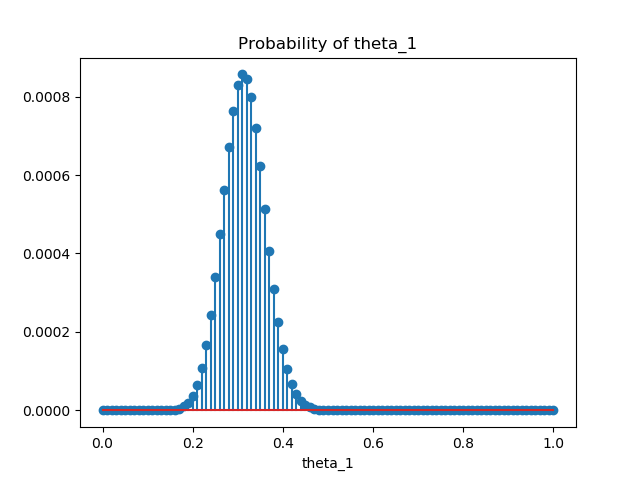
\includegraphics[width = \textwidth]{3.png}
            \caption{Plot of probability distribution of $theta_1$}
            \label{fig:21}
        \end{subfigure}
        \begin{subfigure}{0.8\textwidth}
            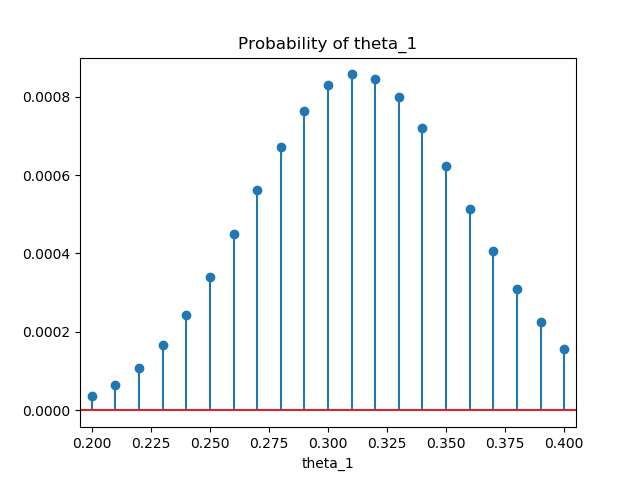
\includegraphics[width = \textwidth]{4.png}
            \caption{Plot of probability distribution of $theta_1$
            , enlarged from $\theta_1=20$ to $\theta_1=40$}
            \label{fig:22}
        \end{subfigure}
        \caption{Probability distribution of $theta_1$}
        \label{fig:2}
    \end{figure}
    Figure \ref{fig:2} is the probability distribution of $\theta_1$.
 
    \item Let $\epsilon=0.02$. Answer using the probability distribution computed
    previously
    \begin{lstlisting}
e = 0.02
print('P{Absolute Error > 0.02} =',\
    sum(theta[i] for i in np.where(abs(x - p) > e)[0]))
print('P{Related Error > 0.02} =',\
    sum(theta[i] for i in np.where(abs(((x - p) / p)) > e)[0]))
    \end{lstlisting}
    \begin{align*}
        \delta_{abs} &= P[|\theta_1^{ML} - \theta_1| > \epsilon] &&= 0.6671038038886307 \\
        \delta_{rel} &= P[|\frac{\theta_1^{ML} - \theta_1}{\theta_1}| > \epsilon] &&= 0.829757447824191 
    \end{align*}
    
    \item For $\epsilon = 0, 0.005, 0.001,\cdots, 1$ plot the graph of 
    $\delta_{abs} = P[|\theta_1^{ML} - \theta_1| > \epsilon]$ vs $\epsilon$.
    Is the function $\delta(\epsilon)$ monotonically increasing, decreasing or neither?
    \begin{lstlisting}
i = 0
epsilons = np.arange(0, 1, step=0.005)
delta = [0]*len(epsilons)
for e in epsilons:
    delta[i] = sum(theta[i] for i in np.where(abs(x - p) > e)[0])
    i = i + 1
plt.plot(epsilons, delta)
plt.xlabel('epsilon')
plt.title('Delta(epsilon) vs. epsilon')
plt.show()
    \end{lstlisting}
    \begin{figure}[h]
        \center
        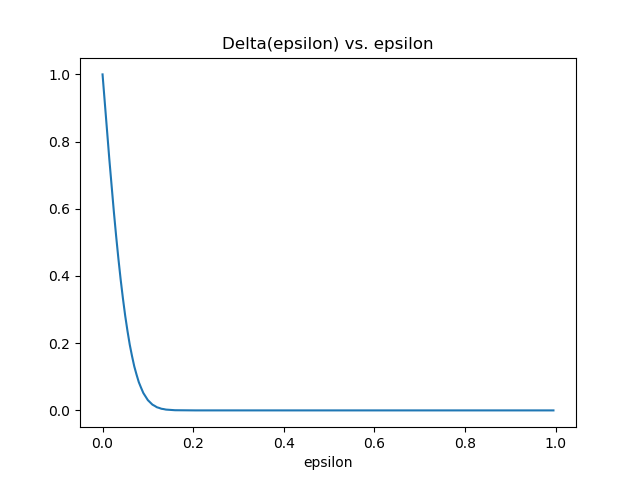
\includegraphics[width=0.8\textwidth]{5.png}
        \caption{$\delta(\epsilon)$ vs. $\epsilon$}
        \label{fig:3}
    \end{figure}

    From the figure \ref{fig:3}, we can clearly see that the function
    $\delta(\epsilon)$ is monotonically decreasing(non-increasing).

    \item Simulate tossing the coin with $\theta_1=0.3141$, $n=100$ times
    and compute $\theta_1^{ML}$. What is the value you $\theta_1^{ML}$
    have obtained, and what are the absolute and relative error?
    \begin{lstlisting}
# Simulation
np.random.seed(999)
y = sum(np.random.binomial(1, p, n))
theta = y / n
print(theta - p)
print((theta - p) / p)
    \end{lstlisting}
    \begin{spverbatim}
    Absolute Error of Simulation =  0.08590000000000003
    Relative Error of Simulation =  0.27347978350843694
    \end{spverbatim}

    Further, I have made 1000 observations to see the behavior of simulated 
    $\theta_1$
    \begin{lstlisting}
observations = 1000

yy = np.repeat(0, n+1)
for k in range(observations):
    yi = sum(np.random.binomial(1, p, n))
    yy[yi] = yy[yi] + 1

theta = [yy[i] / (n*observations) for i in range(0, n+1)]
x = np.arange(0, 1.01, step=0.01)
plt.stem(x, theta)
plt.xlabel('Simulated theta_1')
plt.title('Probability distribution of simulated theta_1')
plt.show()

e = 0.02
print('P{Absolute Error > 0.02}=',\
        sum(theta[i] for i in np.where(abs(x - p) > e)[0]))
print('P{Related Error > 0.02}=',\
        sum(theta[i] for i in np.where(abs((x - p) / p) > e)[0]))
    \end{lstlisting}
    \begin{figure}[h]
        \center
        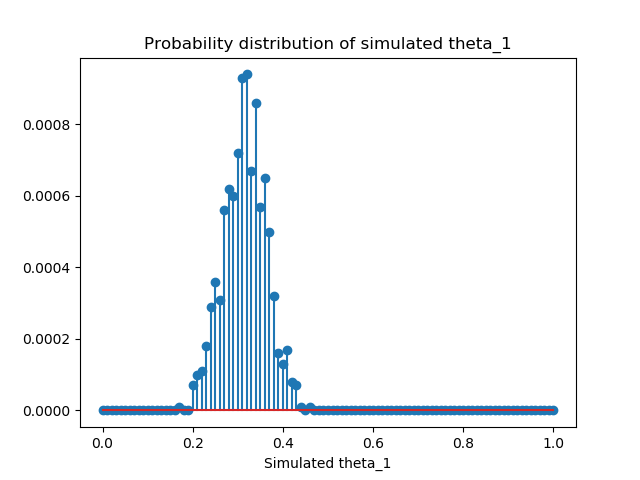
\includegraphics[width=0.8\textwidth]{6.png}
        \caption{Probability distribution of simulated $\theta_1$}
        \label{fig:4}
    \end{figure}
    \begin{spverbatim}
    P{Absolute Error > 0.02} = 0.6730000000000002
    P{Related Error > 0.02} = 0.8120000000000003
    \end{spverbatim}

    \item Let $\theta_1^{'}$ have the value $\theta_1^{ML}$ of the previous
    question. Repeat Question 3-6 using "the guess $\theta_1^{'}$ instead
    of "the truth" $\theta$.
    \begin{lstlisting}
#==========================================================#
# Use the guess theta
p = theta_1

log_P = [0]*101
for i in range(0, 101): # using ln-gamma to avoid overflow
    log_P[i] = math.log(math.gamma(n+1)) - math.log(math.gamma(i+1)) -\
            math.log(math.gamma(n-i+1)) + i*math.log(p) + (n-i)*math.log(1-p)
y = [math.exp(log_P[i]) for i in range(len(log_P))]
plt.stem(y)
plt.xlabel('k')
plt.title('Probability of observing outcome 1 with k times')
plt.show()

theta = [y[i] / n for i in range(0, n+1)]
x = np.arange(0, 1.01, step=0.01)
plt.stem(x, theta)
plt.xlabel('theta_1')
plt.title('Probability of theta_1')
plt.show()

e = 0.02
print('P{Absolute Error > 0.02}=',\
        sum(theta[i] for i in np.where(abs(x - p) > e)[0]))
print('P{Related Error > 0.02}=',\
        sum(theta[i] for i in np.where(abs((x - p) / p) > e)[0]))

i = 0
epsilons = np.arange(0, 1, step=0.005)
delta = [0]*len(epsilons)
for e in epsilons:
    delta[i] = sum(theta[i] for i in np.where(abs(x - p) > e)[0])
    i = i + 1
plt.plot(epsilons, delta)
plt.xlabel('epsilon')
plt.title('Delta(epsilon) vs. epsilon')
plt.show()

# Simulation
np.random.seed(999)
y = sum(np.random.binomial(1, p, n))
theta = y / n
print('Absolute Error of Simulation = ', abs(theta - p))
print('Relative Error of Simulation = ', abs((theta - p) / p))
    \end{lstlisting}
    \begin{figure}[h]
        \center
        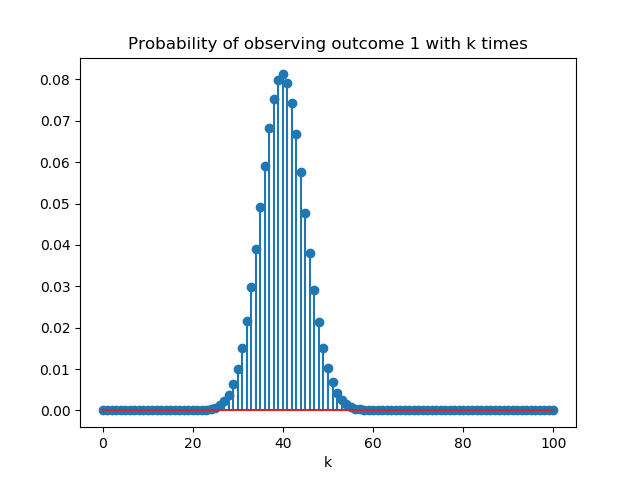
\includegraphics[width=0.8\textwidth]{7.png}
        \caption{Probability distribution of outcome 1 using guess $\theta$}
        \label{fig:5}
    \end{figure}
    \begin{figure}[h]
        \center
        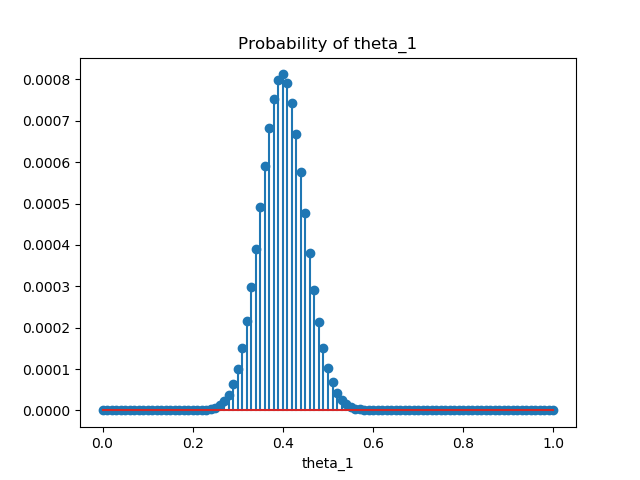
\includegraphics[width=0.8\textwidth]{8.png}
        \caption{Probability distribution of $\theta_1$ using guess $\theta$}
        \label{fig:6}
    \end{figure}
    \begin{figure}[h]
        \center
        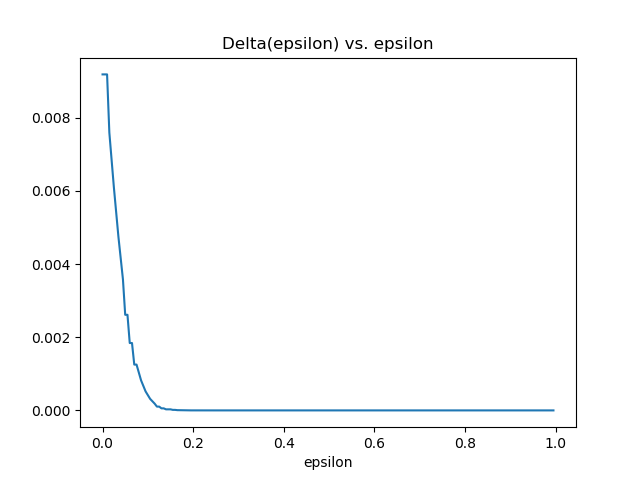
\includegraphics[width=0.8\textwidth]{9.png}
        \caption{$\delta(\epsilon)$ vs. $\epsilon$ using guess $\theta$}
        \label{fig:7}
    \end{figure}
    From the figure \ref{fig:7}, we can see that the function is still
    monotonically decreasing(non-increasing). And for the error part,
    \begin{spverbatim}
    P{Absolute Error > 0.02}= 0.00685447787126666
    P{Related Error > 0.02}= 0.009187808550038788
    Absolute Error of Simulation =  0.06999999999999995
    Relative Error of Simulation =  0.17499999999999988
    \end{spverbatim}
    \end{enumerate}
    
    \section{Problem 5- Rare outcomes and data set size}
    \begin{enumerate}
    \item What is the probability that the outcome sequence contains no 1's?
    \begin{equation*}
        P(n_1 = 0) = \theta_1^0 * (1 - \theta_1)^{n}
    \end{equation*}
    \item What is the probability that the outcome sequence contains a single 1?
    \begin{equation*}
        P(n_1 = 1) = \theta_1^1 * (1 - \theta_1)^{n-1}
    \end{equation*}
    \item Solve $p_0 = p_1$
    \begin{align*}
        p_0                             &\approx p_1 \\
        P(n_1 = 0)                      &= P(n_1 = 0) + \epsilon\\
        \theta_1^0 * (1-\theta_1)^{n}   &= \theta_1^1 * (1-\theta_1)^{n-1} + \epsilon\\
        (1-\theta_1)^{n}                &= \theta_1^1 * (1-\theta_1)^{n-1} + \epsilon
    \end{align*}
    Say, the tolerance to be $\epsilon = 10^{-10}$
    
    \item Compute the above n for $\theta_1 = 10^{-3}, 10^{-4}, 10^{-5}$.
    \end{enumerate}
\end{document}
    